\section{Rapidité des systèmes asservis}
\marginnote{\textbf{Frédéric Mazet}, \textit{Cours d'automatique de deuxième année}, Lycée Dumont Durville, Toulon.}
\marginnote{\textbf{Florestan Mathurin}, \textit{Stabilité des SLCI}, Lycée Bellevue, Toulouse \url{http://florestan.mathurin.free.fr/}.}

%Florestan Mathurin, %\textit{Stabilité des SLCI, Lycée Bellevue, Toulouse}, 
%\url{http://florestan.mathurin.free.fr/}.
%}

\subsection{Rappel : critère de rapidité dans le domaine temporel}

\subsubsection{Temps de réponse à 5\%}

\begin{marginfigure}
\centering
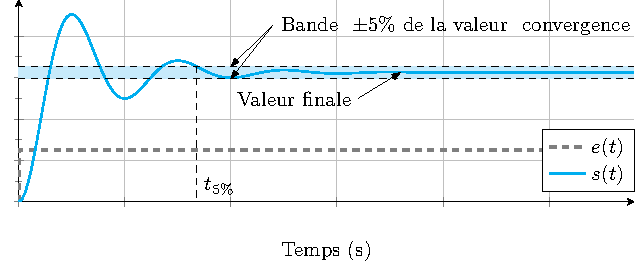
\includegraphics[width=\linewidth]{perf}
\end{marginfigure}

\begin{methode}[Détermination du temps de réponse]%à $n\%$  -- En pratique $n=5$]
En pratique, on détemine le temsp de réponse à 5\%.
\begin{enumerate}
\item Tracer sur le même graphe la consigne $e(t)$ et la réponse du système
$s(t)$.
\item Tracer la droite correspondant à la valeur asymptotique de $s(t)$.
\item Tracer la bande correspondant à une variation de $\pm n\%$ de la valeur
asymptotique.
\item Relever la dernière valeur à partir de laquelle $s(t)$ coupe la bande et
n'en sort plus.
\end{enumerate}
\end{methode}

\begin{resultat}
Plus le temps de réponse à 5\% d'un système est petit, plus le régime transitoire disparaît rapidement. 
\end{resultat}


\begin{marginfigure}[1cm]
\centering
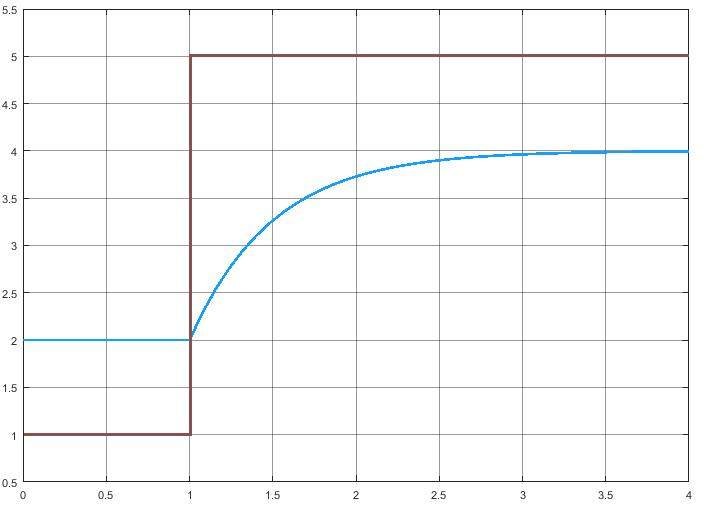
\includegraphics[width=\linewidth]{tr.jpg}
\end{marginfigure}

\begin{exemple}[Donner le temps de réponse à 5\% de la réponse à un échelon donné dans la figure suivante.]
Les pièges du temps de réponse à 5\% :
\begin{itemize}
\item le temps de réponse à 5\% se mesure à plus ou moins 5\% de la sortie (et pas de l'entrée). Ainsi, si le système est stable, le temps de réponse n'est \textbf{jamais l'infini};
\item si le signal ne part pas de 0 (en ordonnée), il faut réaliser la bande à $S_0+\Delta s \pm 0.05\Delta s$;
\item si le signal ne part pas de 0 (en abscisse), il faut tenir compte du décalage des temps.
\end{itemize}

\end{exemple}

\subsubsection{Temps de montée}


\begin{marginfigure}
\centering
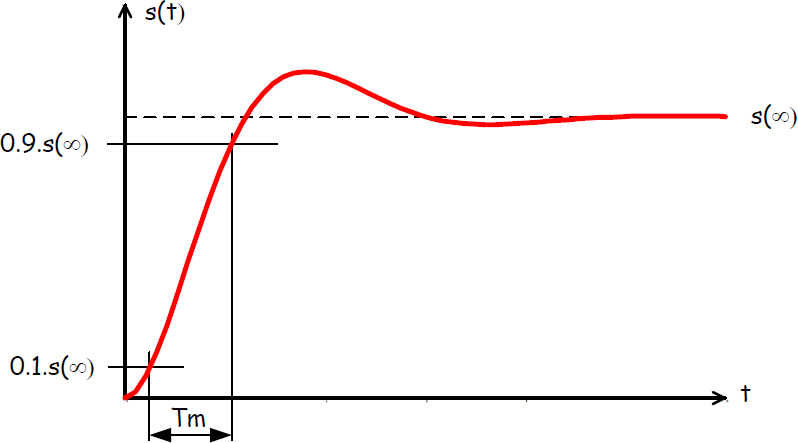
\includegraphics[width=\linewidth]{tm}
\end{marginfigure}

Pour caractériser la rapidité d'un système, on peut aussi utiliser le temps de montée. Il s'agit du temps nécessaire pour passer de 10\% à 90\% de la valeur finale. Ce temps de montée caractériser la << vivacité >> d'un système. 

\subsection{Rapidité des systèmes d'ordre 1 et d'ordre 2}
\subsubsection{Systèmes d'ordre 1}
Pour un système du premier ordre, le temps de réponse à 5\% est donné par $3\tau$.
\begin{resultat}
Pour un système du premier ordre, plus la constante de temps est petite, plus le système est rapide.
\end{resultat}

Soit un système du premier ordre bouclé avec un retour unitaire. L'expression de la FTBF est donnée par $\text{FTBF}(p)=\dfrac{K}{1+\tau p + K}$. La constante de temps est alors $\tau_{\text{BF}}=\dfrac{\tau}{1+K}$. 

\begin{resultat}
Pour un système du premier ordre bouclé (avec un retour unitaire), plus le gain statique est grand, plus le système est rapide. 
\end{resultat}

\subsubsection{Systèmes d'ordre 2}
\begin{marginfigure}
\centering
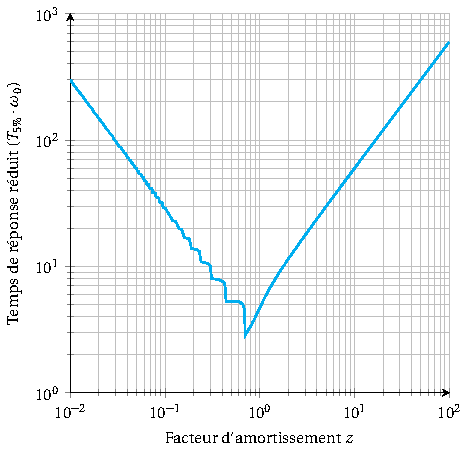
\includegraphics[width=\linewidth]{image7}
\end{marginfigure}

\begin{resultat}
Pour un système du second, à $\xi$ constant, plus la pulsation propre est grande, plus le système est rapide. 
\end{resultat} 


Soit un système du deuxième ordre bouclé avec un retour unitaire. En déterminant les caractéristiques de la FTBF, on obtient $K_{\text{BF}}=\dfrac{K}{1+K}$, $\omega_{\text{BF}}=\omega_0\sqrt{1+K}$, $\xi_{\text{BF}}=\dfrac{\xi}{\sqrt{1+K}}$.



\begin{resultat}
\begin{itemize}
\item L'augmentation du gain de FTBO augmente la pulsation de la FTBF. 
\item L'augmentation du gain de FTBO diminue le coefficient d'amortissement. Suivant la valeur de $\xi{\text{BF}}$ le système peut devenir plus ou moins rapide.  
\end{itemize}
\end{resultat}



\subsection{Résultats dans le diagramme de Bode}


\begin{marginfigure}
\centering
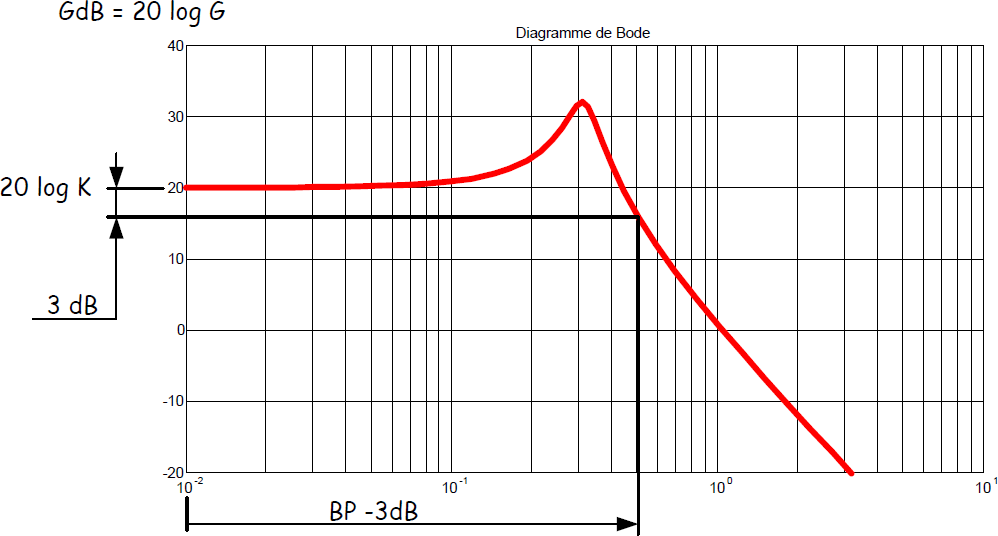
\includegraphics[height=4.5cm]{bandepassante}
\end{marginfigure}

\begin{resultat}
Plus la bande passante d'un système est élevée, plus le système est rapide.
\end{resultat}


\begin{marginfigure}[-2cm]
\centering
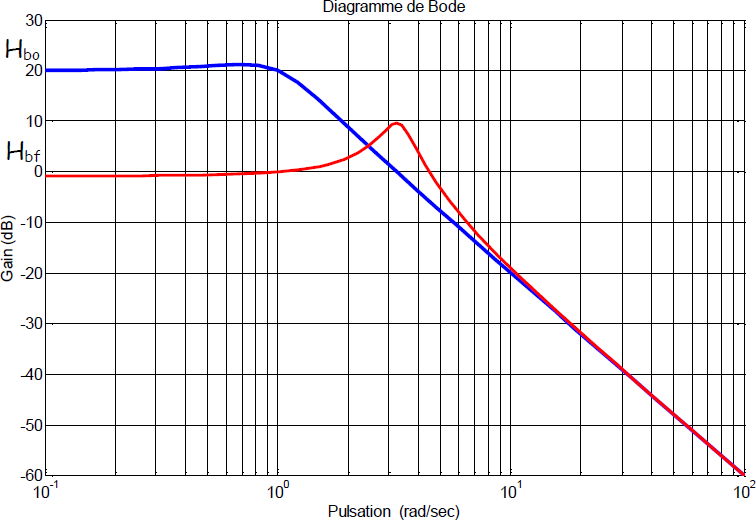
\includegraphics[height=4.5cm]{bobf}
\end{marginfigure}

\begin{resultat}
Plus la pulsation de coupure à \SI{0}{dB} de la boucle ouverte est grande, plus le système asservi est rapide.
\end{resultat}







%\begin{thebibliography}{2}
%   \bibitem[1]{ref1} Frédéric Mazet, {\it Cours d'automatique de deuxième année, Lycée Dumont Durville, Toulon.}
%      \bibitem[2]{ref2} Florestan Mathurin, {\it Stabilité des SLCI, Lycée Bellevue, Toulouse, \url{http://florestan.mathurin.free.fr/}.}
%\end{thebibliography}
